%GNUPLOT: LaTeX picture with Postscript
\begin{picture}(0,0)%
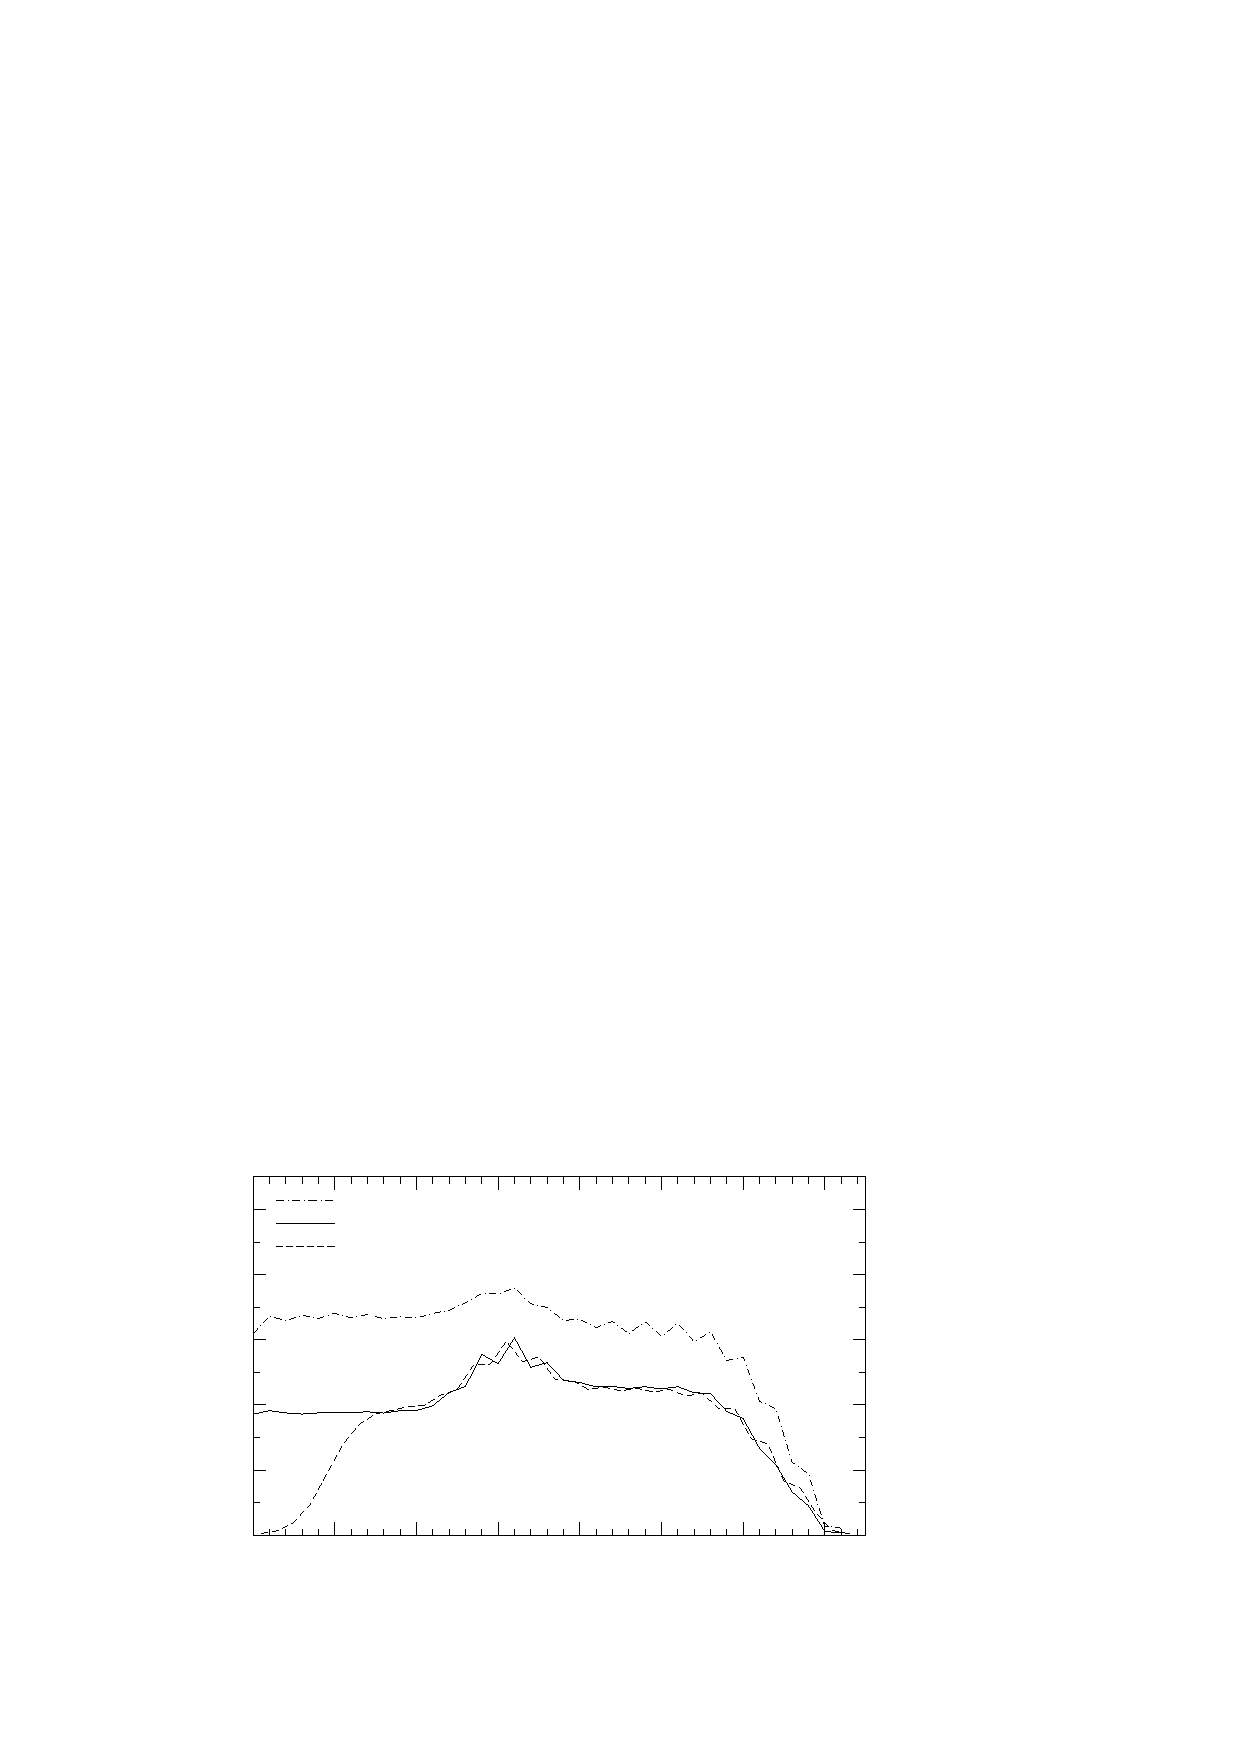
\includegraphics{borderlength}%
\end{picture}%
\begingroup
\setlength{\unitlength}{0.0200bp}%
\begin{picture}(18000,10800)(0,0)%
\put(2200,1650){\makebox(0,0)[r]{\strut{} 0}}%
\put(2200,3214){\makebox(0,0)[r]{\strut{} 0.2}}%
\put(2200,4777){\makebox(0,0)[r]{\strut{} 0.4}}%
\put(2200,6341){\makebox(0,0)[r]{\strut{} 0.6}}%
\put(2200,7905){\makebox(0,0)[r]{\strut{} 0.8}}%
\put(2200,9468){\makebox(0,0)[r]{\strut{} 1}}%
\put(2475,1100){\makebox(0,0){\strut{} 0}}%
\put(4435,1100){\makebox(0,0){\strut{} 10}}%
\put(6395,1100){\makebox(0,0){\strut{} 20}}%
\put(8355,1100){\makebox(0,0){\strut{} 30}}%
\put(10315,1100){\makebox(0,0){\strut{} 40}}%
\put(12275,1100){\makebox(0,0){\strut{} 50}}%
\put(14235,1100){\makebox(0,0){\strut{} 60}}%
\put(16195,1100){\makebox(0,0){\strut{} 70}}%
\put(550,5950){\rotatebox{90}{\makebox(0,0){\strut{}border length / number of probes}}}%
\put(9825,275){\makebox(0,0){\strut{}masking step}}%
\put(4700,9675){\makebox(0,0)[l]{\strut{}E.Coli 1.0 Genome Antisense}}%
\put(4700,9125){\makebox(0,0)[l]{\strut{}Human Genome U95 A}}%
\put(4700,8575){\makebox(0,0)[l]{\strut{}Human Genome U133 Plus 2.0}}%
\end{picture}%
\endgroup
\endinput
